%%%%%%%%%%%%%%%%%%%%%%%%%%%%%%%%%%%%%%%%%%%%%%%%%%%
\begin{frame}
  \begin{center}
    {\Large CNN with TensorFlow}
    
  \end{center}
\end{frame}

%%%%%%%%%%%%%%%%%%%%%%%%%%%%%%%%%%%%%%%%%%%%%%%%%%%
\begin{frame}[fragile] \frametitle{TensorFlow}


\begin{itemize}
\item One set of wts and biases each layer.
\item Conv2D used to specify layer
\item Scans images in both direction
\item Relu for hidden layers.
\item Reshape flattens
\item Accuracy is 98.9\% but shows over-fitting.
\item Use dropouts in fully connected as neurons are more. 
\item Bigger windows more output channels.
\end{itemize}

\end{frame}

%%%%%%%%%%%%%%%%%%%%%%%%%%%%%%%%%%%%%%%%%%%%%%%%%%%%
%\begin{frame}[fragile] \frametitle{Convolution Network}
%%
%%\adjustbox{valign=t}{
%%\begin{minipage}{0.45\linewidth}
%\begin{itemize}
%\item Image is input
%\item $W_1$ has window of $5x5$, with channel 1 (mono chrome), wt sets 4
%\item With stride 2, image halved14x14. Previous wt set 4, become input channels now.
%\item Last is fully connected to 10 outputs
%\end{itemize}
%%\end{minipage}
%%}
%%\hfill
%%\adjustbox{valign=t}{
%%\begin{minipage}{0.45\linewidth}
%\begin{center}
%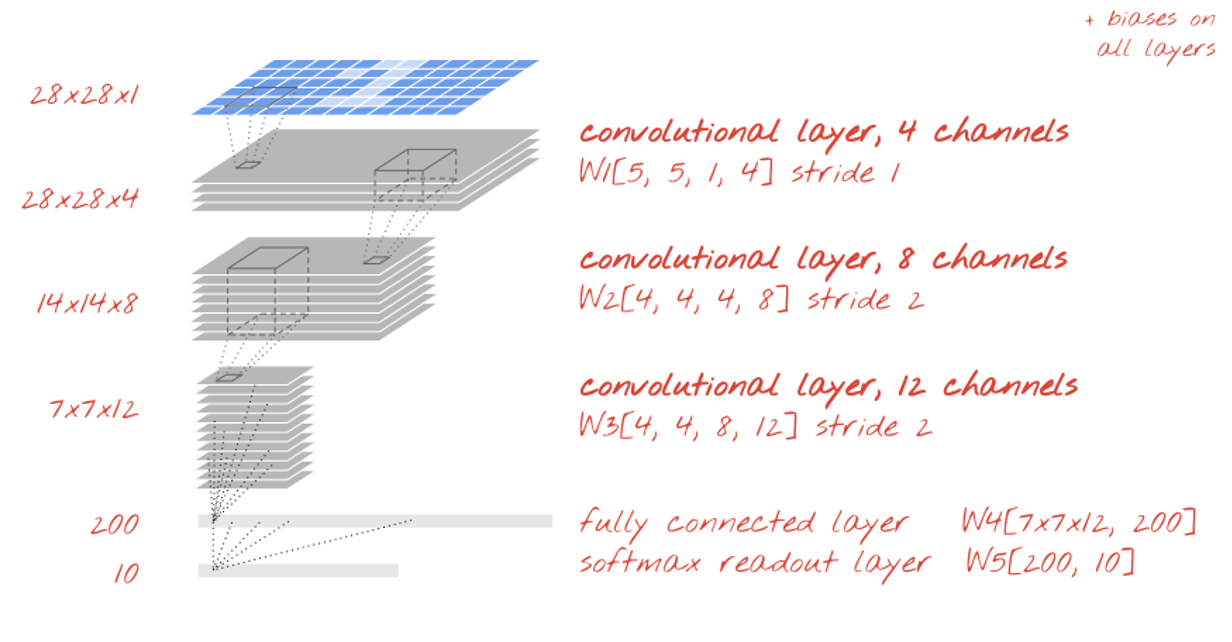
\includegraphics[width=0.8\linewidth,keepaspectratio]{cnnchannel}
%\end{center}
%%\end{minipage}
%%}
%
%\end{frame}
%
%
%%%%%%%%%%%%%%%%%%%%%%%%%%%%%%%%%%%%%%%%%%%%%%%%%%%%
%\begin{frame}[fragile] \frametitle{Convolution layer}
%
%\adjustbox{valign=t}{
%\begin{minipage}{0.45\linewidth}
%\begin{itemize}
%\item Color Images shown as 3 stacks (3 RGB values for each pixel, vertically)
%\item One neuron will be doing weighted sum of X (small patch pixel values)
%\item Next neuron, will take  next patch keeping the weights same.
%\item Once one set of weights is complete, use second set (shown in grey), called output channels
%\end{itemize}
%\end{minipage}
%}
%\hfill
%\adjustbox{valign=t}{
%\begin{minipage}{0.45\linewidth}
%\begin{center}
%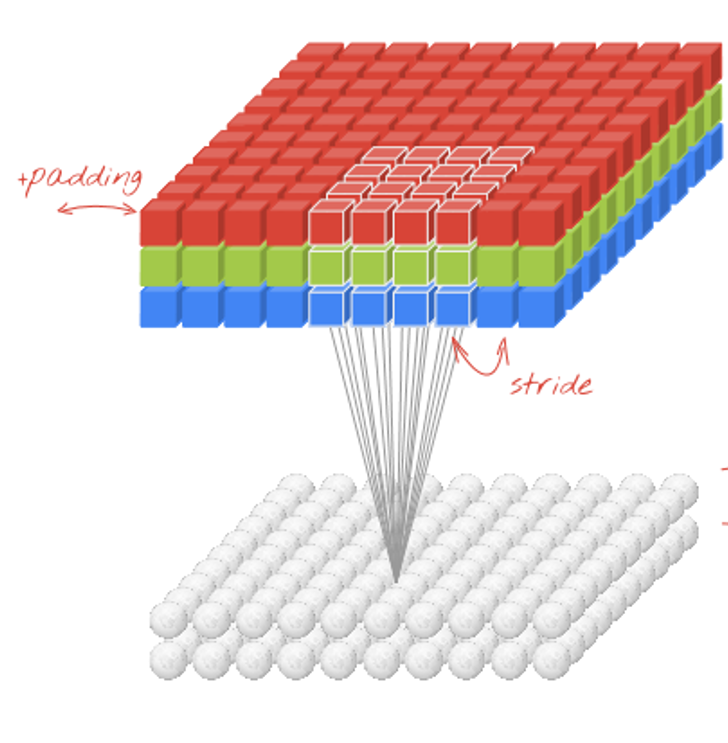
\includegraphics[width=\linewidth,keepaspectratio]{convlayer}
%\end{center}
%\end{minipage}
%}
%
%\end{frame}
%
%
%%%%%%%%%%%%%%%%%%%%%%%%%%%%%%%%%%%%%%%%%%%%%%%%%%%%
%\begin{frame}[fragile] \frametitle{Convolutional Layer Channels}
%
%\begin{center}
%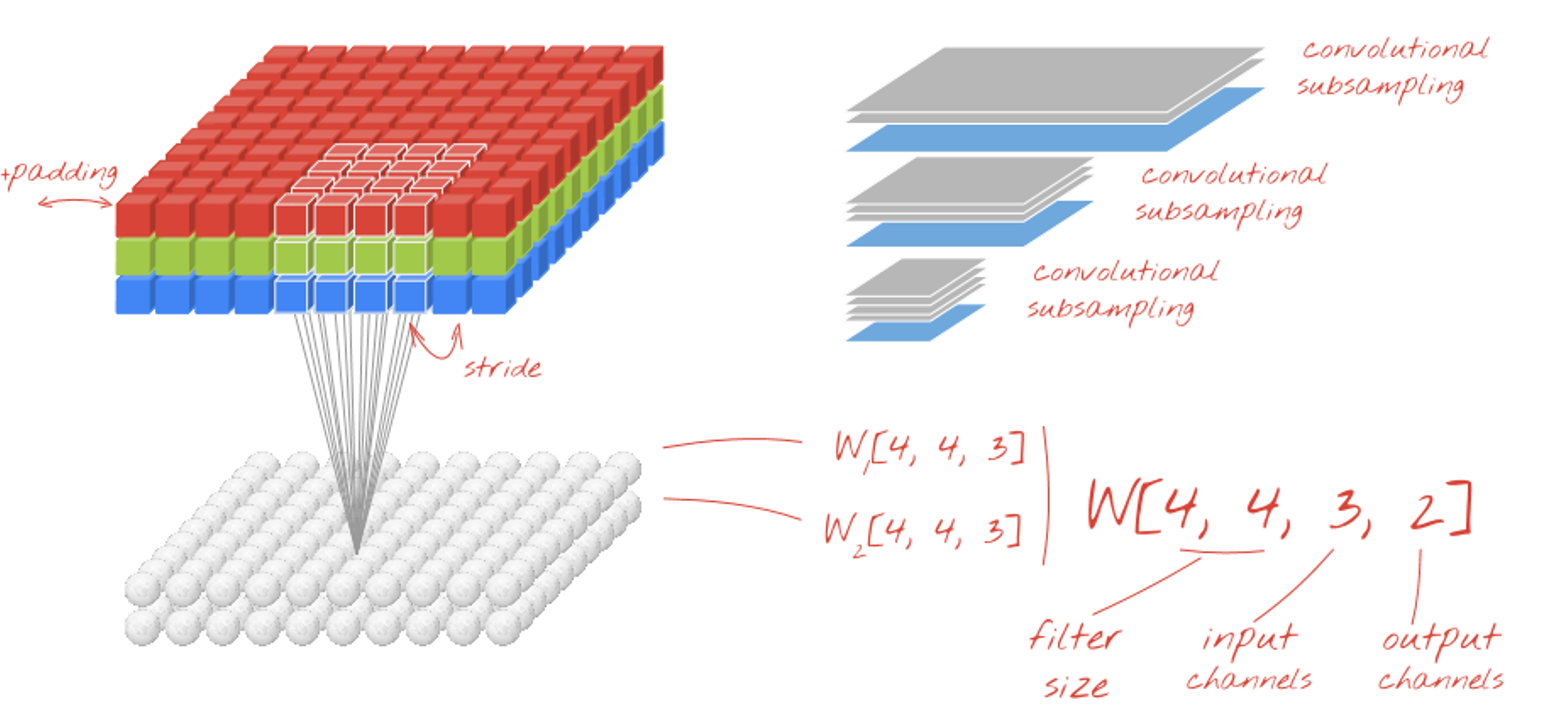
\includegraphics[width=\linewidth,keepaspectratio]{convlayerarray}
%\end{center}
%\end{frame}
%
%%%%%%%%%%%%%%%%%%%%%%%%%%%%%%%%%%%%%%%%%%%%%%%%%%%%
%\begin{frame}[fragile] \frametitle{Convolution parameters}
%
%\adjustbox{valign=t}{
%\begin{minipage}{0.45\linewidth}
%\begin{itemize}
%\item Image window: $4x3$
%\item Channels: 3 (RGB)
%\item Weight sets, output channels: 2
%\begin{itemize}
%\item $W_1 : [4,4,3]$
%\item $W_2: [4,4,3]$
%\item Combined: $W:[4,4,3,2]$
%\end{itemize}
%\item Stride: jumps between window
%\item Padding: extra values at edges
%\end{itemize}
%\end{minipage}
%}
%\hfill
%\adjustbox{valign=t}{
%\begin{minipage}{0.45\linewidth}
%\begin{itemize}
%\item Finally we want 10 outputs (digits). How to bring from so many weights to 10, down?
%\item Subsampling: Takes 4 outputs (2x2), takes max, and passes it to the next layer.
%\item With each layer, image size reduces proportionately
%\end{itemize}
%\end{minipage}
%}
%
%\end{frame}
%
%
%
%%%%%%%%%%%%%%%%%%%%%%%%%%%%%%%%%%%%%%%%%%%%%%%%%%%%
%\begin{frame}[fragile] \frametitle{TensorFlow}
%
%\begin{center}
%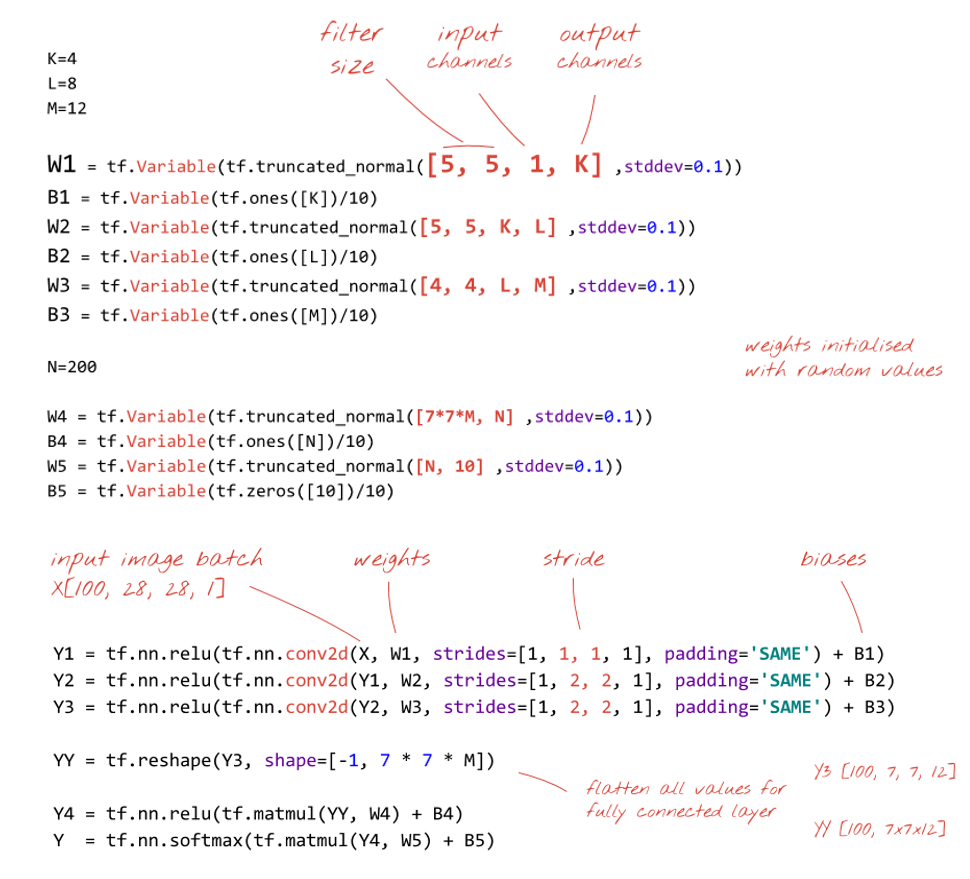
\includegraphics[width=0.7\linewidth,keepaspectratio]{cnntf}
%\end{center}
%
%\end{frame}
%
%
%%%%%%%%%%%%%%%%%%%%%%%%%%%%%%%%%%%%%%%%%%%%%%%%%%%%
%\begin{frame}[fragile] \frametitle{Better network}
%
%99.3\%
%
%\begin{center}
%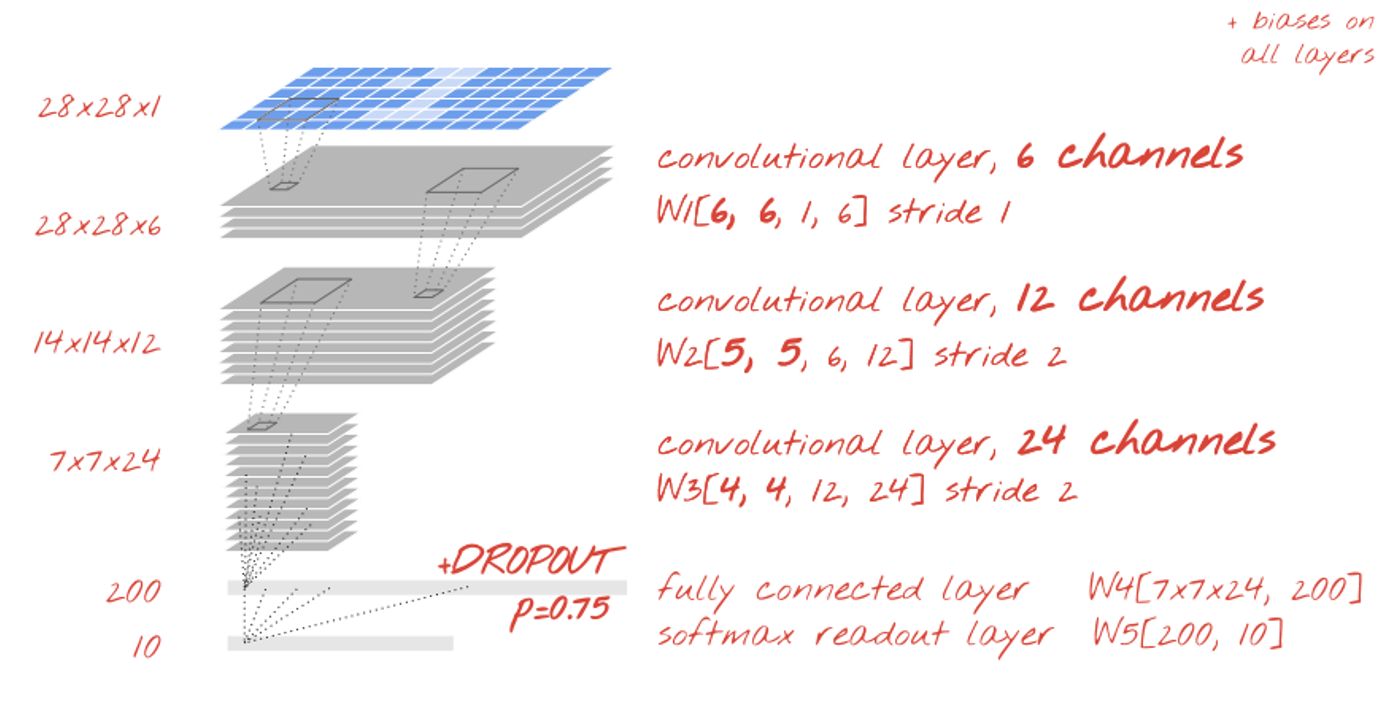
\includegraphics[width=\linewidth,keepaspectratio]{cnnnn}
%\end{center}
%
%\end{frame}
%

%%%%%%%%%%%%%%%%%%%%%%%%%%%%%%%%%%%%%%%%%%%%%%%%%%%
\begin{frame}[fragile] \frametitle{Load the training data, using MNIST}

\begin{center}
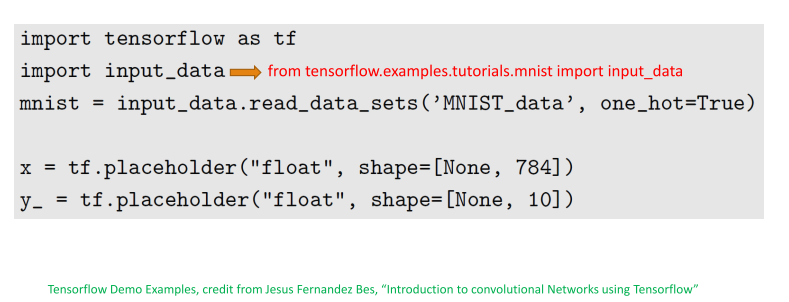
\includegraphics[width=\linewidth,keepaspectratio]{cnntf1}
\end{center}
\end{frame}


%%%%%%%%%%%%%%%%%%%%%%%%%%%%%%%%%%%%%%%%%%%%%%%%%%%
\begin{frame}[fragile] \frametitle{Weight Initialization}

\begin{center}
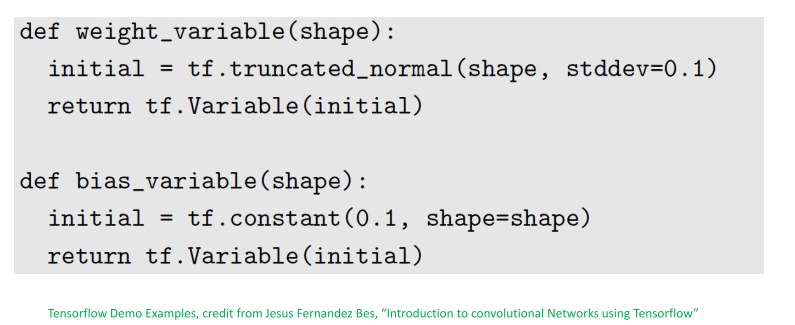
\includegraphics[width=\linewidth,keepaspectratio]{cnntf2}
\end{center}
\end{frame}

%%%%%%%%%%%%%%%%%%%%%%%%%%%%%%%%%%%%%%%%%%%%%%%%%%%
\begin{frame}[fragile] \frametitle{Convolution and Pooling}

\begin{center}
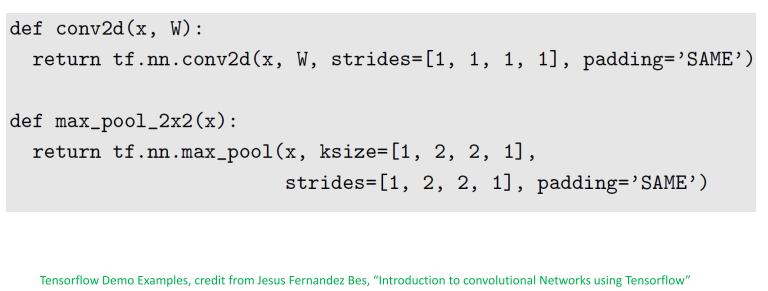
\includegraphics[width=\linewidth,keepaspectratio]{cnntf3}
\end{center}
\end{frame}

%%%%%%%%%%%%%%%%%%%%%%%%%%%%%%%%%%%%%%%%%%%%%%%%%%%
\begin{frame}[fragile] \frametitle{First Convolutional Layer}

\begin{center}
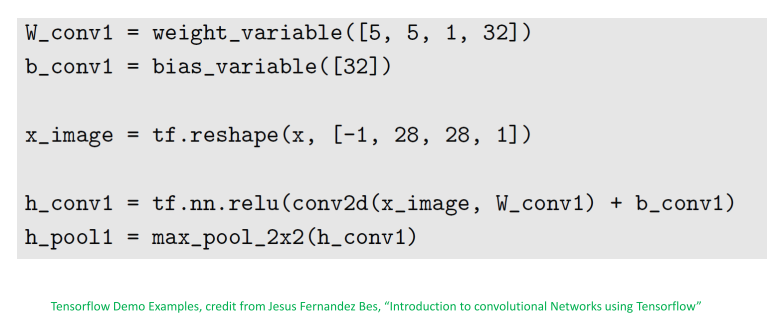
\includegraphics[width=\linewidth,keepaspectratio]{cnntf4}
\end{center}
\end{frame}


%%%%%%%%%%%%%%%%%%%%%%%%%%%%%%%%%%%%%%%%%%%%%%%%%%%
\begin{frame}[fragile] \frametitle{Second Convolutional Layer}

\begin{center}
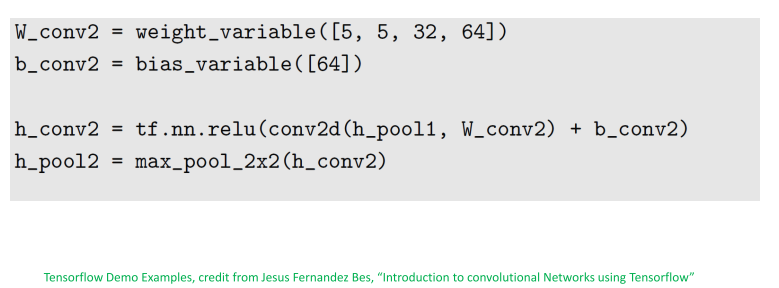
\includegraphics[width=\linewidth,keepaspectratio]{cnntf5}
\end{center}
\end{frame}


%%%%%%%%%%%%%%%%%%%%%%%%%%%%%%%%%%%%%%%%%%%%%%%%%%%
\begin{frame}[fragile] \frametitle{Fully Connected Layer}

\begin{center}
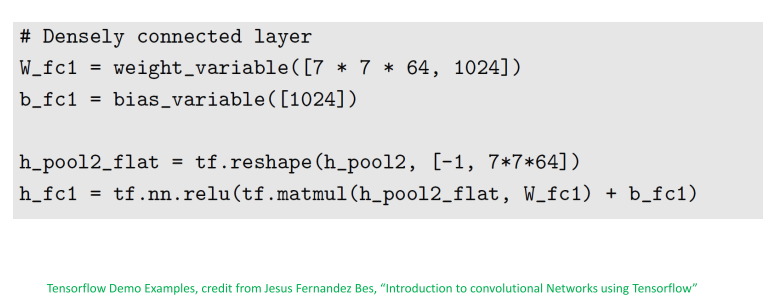
\includegraphics[width=\linewidth,keepaspectratio]{cnntf6}
\end{center}
\end{frame}

%%%%%%%%%%%%%%%%%%%%%%%%%%%%%%%%%%%%%%%%%%%%%%%%%%%
\begin{frame}[fragile] \frametitle{Dropout}

\begin{center}
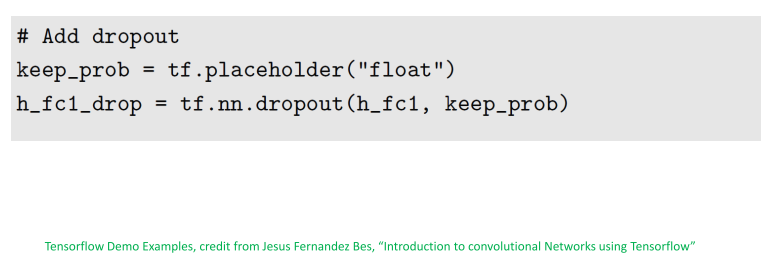
\includegraphics[width=\linewidth,keepaspectratio]{cnntf7}
\end{center}
\end{frame}

%%%%%%%%%%%%%%%%%%%%%%%%%%%%%%%%%%%%%%%%%%%%%%%%%%%
\begin{frame}[fragile] \frametitle{Readout Layer}

\begin{center}
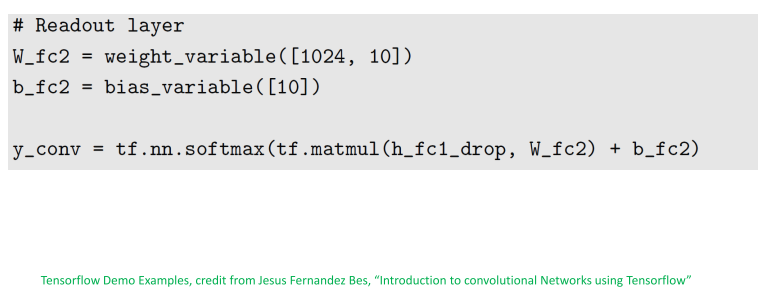
\includegraphics[width=\linewidth,keepaspectratio]{cnntf8}
\end{center}
\end{frame}

%%%%%%%%%%%%%%%%%%%%%%%%%%%%%%%%%%%%%%%%%%%%%%%%%%%
\begin{frame}[fragile] \frametitle{Train and Evaluate}

\begin{center}
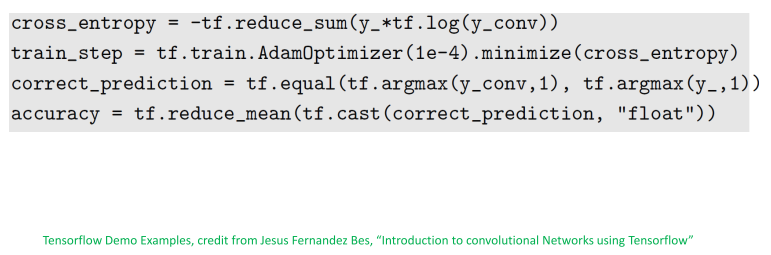
\includegraphics[width=\linewidth,keepaspectratio]{cnntf9}
\end{center}
\end{frame}


%%%%%%%%%%%%%%%%%%%%%%%%%%%%%%%%%%%%%%%%%%%%%%%%%%%
\begin{frame}[fragile] \frametitle{Execute}

\begin{center}
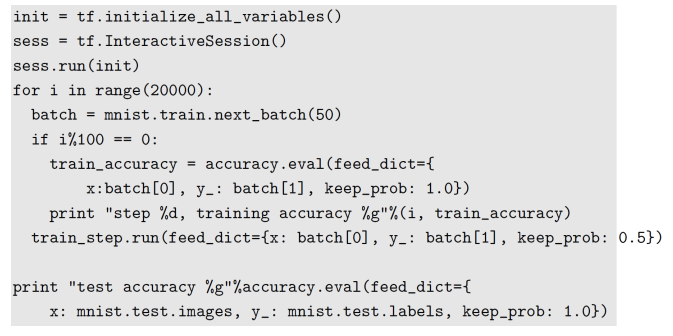
\includegraphics[width=\linewidth,keepaspectratio]{cnntf10}
\end{center}
\end{frame}
